\documentclass{llncs}
\usepackage[ruled,vlined]{algorithm2e}
\usepackage{color,graphicx,epstopdf,changepage,amsmath,multirow}

\SetAlgoCaptionSeparator{.\space}
\renewcommand\AlCapFnt{\normalfont\scshape}
\setlength{\algomargin}{0.7cm}

\title{Comprehensive quality - aware Automated Semantic Web Service Composition}

\author{Chen Wang, Hui Ma, and Aaron Chen}
\institute{School of Engineering and Computer Science,
\\Victoria University of Wellington, New Zealand \\
\email{\{Chen.Wang, Hui.Ma, and Aaron.Chen\}@ecs.vuw.ac.nz }}

\makeatletter
\usepackage[pdfauthor={\@author}, pdftitle={\@title}]{hyperref}
\makeatother

\providecommand{\e}[1]{\ensuremath{\times 10^{#1}}}

\begin{document}

\maketitle

\begin{abstract}
Semantic web service composition has been a prevailing research area in recent years. There are two major governance challenges faced by researchers. One is semantic matchmaking for discovering interoperable web services, which demands a rich “machine understanding” language such as OWL-S (Web Ontology language for Web Services), WSML (Web Service Modeling language, SAWSDL (Semantic Annotations for WSDL and XML Schema). This interaction of web services enables us to pair service functionalities through understanding and reasoning those semantic descriptions. Optimisation problems are another challenge. Many scholars have looked into nonfunctional optimisation problems in QoS-aware web service composition applying AI planning and Evolution Computing techniques. However, it is not sufficient without considering good balance between functional and nonfunctional quality in most scenarios. Therefore, the consideration in these two quality dimensions is a must, so that service composition needs to deal with optimisation problems in both quality of semantic matchmaking and QoS. This paper develops a more applicable way for measuring a proposed comprehensive quality model in both semantic matchmaking and QoS for automated semantic web service composition.
\end{abstract}

\section{Introduction}\label{introduction}
Service-oriented computing (SOC) is a novel computing paradigm that employs services as fundamental elements to achieve agile development of cost-efficient and integratable enterprise applications in heterogeneous environments \cite{papazoglou2003service}. Service Oriented Architecture (SOA) could abstractly realise service-oriented paradigm of computing. This accomplishment has been contributing to the reuse of software components, from functions to units, and from units to services during the development in SOA \cite{booth2004web}. One of the most typical realisations of SOA is \textit{web service}, which is designated as ``modular, self-describing, self-contained applications that are available on the Internet'' \cite{curbera2001web}. Several standards play a significant role in registering, enquiring and grounding web services including particularly UDDI, WSDL and SOAP \cite{fensel2011semantic}.

\textit{Web service composition} pertains to a combination of multiple web services to provide a value-added composite service that accommodates customers' arbitrarily complex requirements. This application is developed by integrating interoperable and collaborative functionalities over heterogeneous systems. Due to the increase in the number of large-scale enterprise applications, the number of Web services has increased dramatically and unprecedentedly, which cause an immense redundancy in functionality in a huge searching space. Therefore, manual and semi-automated web service composition are considered to be less efficient while automated web service composition is deemed to be less human intervention, less time consumption, and high productivity.

Two most notable challenges for web service composition are $(1)$ ensuring interoperability of services and $(2)$ achieving QoS optimisation \cite{fensel2011semantic}. \textit{Interoperability} of web services presents challenge $(1)$ in the dimensions of syntactic and semantics \cite{fensel2011semantic}. The syntactic dimension is covered the XML-based technologies (such as $WSDL$, $SOAP$). The semantics aspect, on the other hand, demands further research. Through semantics given by ontologies \cite{o2005review}, web services understand and better collaborate with each other. Historically, there are many ontologies languages and formats for semantic service descriptions, such as OWL-S \cite{martin2004owl}, WSML \cite{fensel2006enabling}, and SAWSDL \cite{lausen2007semantic}. The logical characteristics in reasoning makes ``machine understanding'' possible through identifying and matching semantic similarity in input/output parameters of web services in heterogeneous environments. The second challenge $(2)$ is related to finding \textit{optimised solutions} to Quality of Service ($QoS$) over composite web services. This problems give birth to \textit{QoS-aware service composition} that considers the composition of service-level agreements \cite {sahai2002automated} manifesting a collection of SLA rules and policies for supporting QoS-based composition.

Existing works on service composition focus mainly addressing two challenges above. One group optimises the quality of compositions under a pre-defined abstract workflow, which is considered to be a \textit{semi-automated Web service composition} approach. Another group attempts to generate a composite plan automatically in discovering and selecting suitable web services, which are deemed to NP-hard \cite{moghaddam2014service}. \textit{Semantic web services composition} is distinguished from the syntactic service composition. Its benefits are presented in eliminating conflicts by the semantic level of web services. In the past few years, substantial works have been done on semantic web service composition \cite{fensel2011semantic,lecue2009optimizing}. However, few works have enabled truely automatic semantic web service composition, where both QoS and quality of semantic match making will be optimised simultaneously. However, customers often prefer a service composition that matches their requirement most with highest QoS.

The overall goal of this paper is to \textit{develop an comprehensive quality-aware automated semantic web service composition that satisfactorily optimises both functional and non-functional requirements}. Particularly, this paper considers the quality of semantic matchmaking quality and QoS and two structural constructs (sequence and parallel) for building optimised composition solution using Particle Swarm Optimisation (PSO). We aim to provide a more applicable and adaptive way to measure semantic matchmaking in automated semantic web service composition. We will achieve three objectives in this work as follows:

\begin{enumerate}
 \item To propose a comprehensive quality model that address QoS and semantic matchmaking quality in considering different matching types associated with corresponding semantic similarity. This approach is consider to be a more applicable and effective way of finding an optimised solution in semantic web service composition.
  
 \item To propose a PSO-based service composition model that utilise the proposed quality model. In PSO, weighted graphs with edges and vertices associated with quality of semantic matchmaking and QoS respectively represent the solutions of semantic web service composition as particles in the searching space, which are decoded from an optimised service queue with the consideration of comprehensive quality.
  
 \item To evaluate the performance of comprehensive quality awareness semantic web service composition by utilising benchmark datasets from Web Services Challenge 2009 (WSC09) \cite{kona2009wsc}.
\end{enumerate}

The remains of this paper are organised as the following: Sect. \ref{background} provides the background on the semantic web service composition, and related works; Sect. \ref{qswsc_approach} presents an overview of comprehensive quality-aware semantic automated web service composition consisting of comprehensive quality evaluation model and PSO-based service composition algorithm; Sect. \ref{experiment_design} describes the experiments conducted to test the effectiveness of proposed model; Sect. \ref{results_analysis} presents and analyses the experiment; Sect. \ref{conclusion} concludes our work.

\section{Related Work} \label{relatedWork}
\textbf{Semantic web service matchmaking}. Substantial work \cite{bansal2016generalized,mier2015integrated,da2016particle,da2015graphevol,yu2013adaptive} on web service composition focused mainly on non-functional requirements consistently neglecting functional requirements. However few researchers addressed both addressed both of them at the same time in web service composition. To the best of our knowledge, \cite{fanjiang2014semantic,lecue2009optimizing} are the papers could be found so far. Semantic matchmaking utilises Description Logic($DL$) \cite{baader2003description} reasoning between input and output parameter concepts of web services to ensure a semantic matchmaking. It is considered be a process consisting of seeking similarity of parameters (i.e., input and output) of web services and mapping between two knowledge representations encoded utilising the ontology \cite{lecue2006formal}.

In \cite{shet2012new}, three approaches are surveyed three approaches regarding the similarity measures using taxonomies: $(1)$ The first one is based on nodes, in which similarity is determined by the information content of the nodes; $(2)$ the second is entirely based on edge, where concept distance in a hierarchy structure is evaluated, and $(3)$ the hybrid approach features a combination of $(1)$ and $(2)$. A new similarity measure based on edge counting in taxonomy is introduced in \cite{shet2012new}, which extends similarity measure defined by Wu and Palmer \cite{wu1994verbs}. Neighbourhood concepts are considered in their model when $\lambda$ = 1 (default value as 0).

In \cite{lecue2009optimizing}, the quality of matchmaking problem is transferred to measure the quality of semantic links $sl_{i,j} \stackrel{.}{=} \langle s_{i}, Sim_{T}(Out\_s_i,In\_s_j),s_{j}  \rangle$, one possible measure is applied for the degree of similarity using Common Description rate of a semantic link, where Extra Description $In_{s_{x}} \setminus Out_{s_{y}}$ and Least common subsume $lcs(Out_{s_i},In_{s_j})$ are required to be pre-calculated. They also chained the web service with five well-known matching types: Exact, Plug-in, Subsume, Intersection, and Disjoint. Therefore, the quality of the semantic link is estimated as quality criteria $q_{m}$ associated with their corresponding quality of vector $q_{cd}$.

However, the weakness of semantic link quality is that calculating Extra description and Least common subsume requires well and completely defined ontology in class, class axioms and properties in OWL2. This makes it difficult to measure semantic matchmaking quality in most semantic web services applications, as it takes unpredictable cost and time for the domain experts to establish required ontology. Additionally, a semi-automated service composition approach is considered in their paper, rather than a fully automated method. In QoS, only cost and time are considered in the optimised problems. Therefore, we introduce a more applicable comprehensive quality model in a fully automated approach.

In \cite{fanjiang2014semantic}, it covers the concerns in both functional and non-functional requirements in design time of semantic-based automatic service composition, where a GA-based approach with four unusual independent fitness functions are designed to solve the problems with these concerns. In details, a sequence of fitness functions are used in the binary selection of chromosomes, rather than a single objective consisting of both functional and non-functional quality. Apart from that, match types are ignored in their quality evaluation of semantic matching.

\textbf{QoS-aware EC approaches}. Evolution Computing techniques are widely used to solve optimisation problem. Genetic Programming (GP) \cite{da2016particle,da2015graphevol} is a typical EC technique to solve automated web service composition. This GP-based approach utilises tree representations, on which service and constructs as represented as terminal nodes and functional nodes respectively. The crossover and mutation operations reproduce various individuals while ensuring the correctness of structure. In \cite{yu2013adaptive}, the author optimises the overall quality of service composition by using a fitness function, which is also liable for the correctness in functionality through penalising infeasible solutions. 

To simplify the checking of constraints for solutions, an indirect PSO-based approach was introduced in \cite{da2016particle}. A general graph is used as representation as particles in their PSO algorithm considering QoS optimisation. However, this solution does not distinguish different matching types and parameter similarity, which could lead to the outputs returned by the selected service that we think may be too general. In fact, customers' perspectives, application domains and ontology granularity all could have significant impacted on the outputs requested by users. In some scenarios, the output returns too broad consequences that have no meaning for the customers, even though those web services selected leads to a very good overall QoS. Therefore, we fill the gap by considering different matching types and the similarity when evaluate an overall quality of web service composition and utilising weighed graphs as different particle representations from \cite{da2016particle}.

\section{Problem Description}\label{problemDes}

The purpose of web service composition is to accomplish an arbitrarily complex task fulfilling customer's requirement, which could be denoted as a composite goal: $Comp.G(F(T_{Input}, T_{Output}), NF(T_{QoS}))$. This overall composite goal is demonstrated in two parts. The first functional part is a given task input or input set to get the desired Task output or output set. It typically refers to users' functional requirement. Another nonfunctional part specifies the acceptable level of composite quality of service. To accomplish the composite goal, two stages are involved: services discovery and service selection. Firstly, service discovery is to find matched web service: $S_{n}(F(S_{Input}, S_{Output}), NF(S_{QoS}))$ from a Service Repository: $S =  \{S_{1}, S_{2},..., S_{n} \}$ with the given $T_{Input}$. If no atomic web service could satisfy the composite goal, a combination of web services will be found concretely to meet $Comp.G$. To ensure the composite solution returns the desired $Comp.G$, we consider a comprehensive quality model for service discovery and selection, where challenges $(1)$ and $(2)$ mentioned in Sect. \ref{introduction} are also addressed in Sect. \ref{qswsc_approach}.

\subsection{Semantic Web Service matchmaking Type}\label{semantic Web service Discovery}
The semantic service matchmaking aims to discover appropriate services from service repository relevant to a customer's functional requests. A semantic web service is defined by $S(F(S_{Input}\in C_{1}, S_{Output}\in C_{2}), NF(S_{QoS}))$ with both Input and Output are linked to concept $C_{1}$ and $C_{2}$ in an ontology ($O$) respectively, satisfying $O=\{C, Taxonomy\}$. A web service matching process is to match the output and input concepts of two services according to the Taxonomy within an Ontology (O). To measure the quality of semantic matchmaking, different matching levels are typically considered in the literature \cite{paolucci2002semantic}. To understand these levels, let us define two web services associated with parameters in a particular domain. $S_{1}$ $(F(S_{Input}\in C_{1}, S_{Outputs}\in C_{2}), NF(S_{QoS}))$ and  $S_{2}$ $(F(S_{Input}\in C_{3}, S_{Output}\in C_{4}), NF(S_{QoS}))$ and an Ontology($O$) with $C_{1},C_{2},C_{3}$, and $C_{4}$. The matching levels to be considered are:

\begin{itemize}
\item \textit{Exact} ($\equiv$): Output of Web service $S_{1}$ and Input of Web service $S_{2}$ are Exact match ($ S_{output} \in S_{1} \equiv S_{input}S_{2}$), if  Concept $C_{2}$ and Concept $C_{3}$ are equivalent.
\item \textit{Plugin} ($\sqsubseteq_{n}$): Output of Web service $S_{1}$ and Input of Web service $S_{2}$ are Plugin match ($S_{output} \in S_{1} \sqsubseteq_{n} S_{input} \in S_{2}$), if  Concept $C_{2}$ is a sub-concept of Concept $C_{3}$, and $n = \{1,2,...,n \}$ presents the levels of children concepts ($n=1$ stands for direct children).
\item \textit{Subsume} ($\sqsupseteq_{n}$): Output of Web service $S_{1}$ and Input of Web service $S_{2}$ are Subsume matched($S_{output} \in S_{1} \sqsupseteq_{n} S_{input} \in S_{2}$), if  Concept $C_{2}$ is a sub-concept of  Concept $C_{3}$, and $n = \{1,2,...,n \}$ presents the levels of parent concepts ($n=1$ stands for direct parent).
\item \textit{Fail} ($\perp$). Output of Web service $S_{1}$ and Input of Web service $S_{2}$ are not matched (Fail) ($S_{output} \in S_{1} \perp S_{input} \in S_{2}$), if none of the previous matches discovered.
\end{itemize}

Note that, to find relevant services for service compositions according to a given goal, we consider Exact, Plugin, Subsume and Fail match types in our paper. Therefore, these matches will be used to discover web service candidates for service composition in our proposed the comprehensive quality-aware model in Sect.\ref{semantic_matchmaking}

\subsection{Quality of Service and Composition Constructs}\label{Quality of Service and Composition Constructs}
Currently, most of the optimisation problems \cite{feng2013dynamic,huang2009effective,ma2015hybrid,da2014graph} in web service composition are focusing on QoS, which covers aspects in non-functional requirements. This problem has been explored in both single objective and multi-objectives optimisation problems. Customers prefer lowest execution cost with highest response time and reliability so that it could be involved as a single objective optimisation problem while cost and reliability of web service are two conflicting objectives that could be optimised simultaneously in multi-objective problem. According to \cite{zeng2003quality}, four most often considered QoS parameters are as follows:
\begin{itemize}
\item \textit{Response time} ($T$) measures the expected delay in seconds between the moment when a request is sent and the moment when the results are received.
\item \textit{Cost} ($C$) is the amount of money that a service requester has to pay for executing the web service
\item \textit{Reliability} ($R$) is the probability that a request is correctly responded within the maximum expected time frame.
\item \textit{Availability} ($A$) is the probability that a web service is accessible.
\end{itemize}
The aggregation value of QoS attributes for web services composition varies with respect to different constructs, which explains how services associated with each other in a service composition \cite{zeng2003quality}. Here we consider two composite constructs: sequence and parallel constructs, in building the composite flow. The QoS calculation models are described as follows:

\begin{figure}[h]
\centerline{
\fbox{
\begin{tabular}{p{0.6\linewidth}}
\space\hfill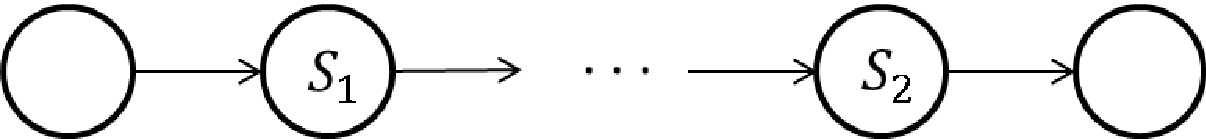
\includegraphics[width=2in]{sequence.pdf}\hfill\space\\[0.2cm]
$T=\sum\limits^m_{n=1}t_n$ \hfill $C=\sum\limits^m_{n=1}c_n$ \hfill
$A=\prod\limits^m_{n=1}a_n$ \hfill $R=\prod\limits^m_{n=1}r_n$
\end{tabular}}}
\caption{Sequence construct and calculation of its QoS properties
\cite{yu2013adaptive}.}
\label{sequence}
%\end{figure}
\vspace{0.3cm}
%\begin{figure}
\centerline{
\fbox{
\begin{tabular}{p{0.6\linewidth}}
\space\hfill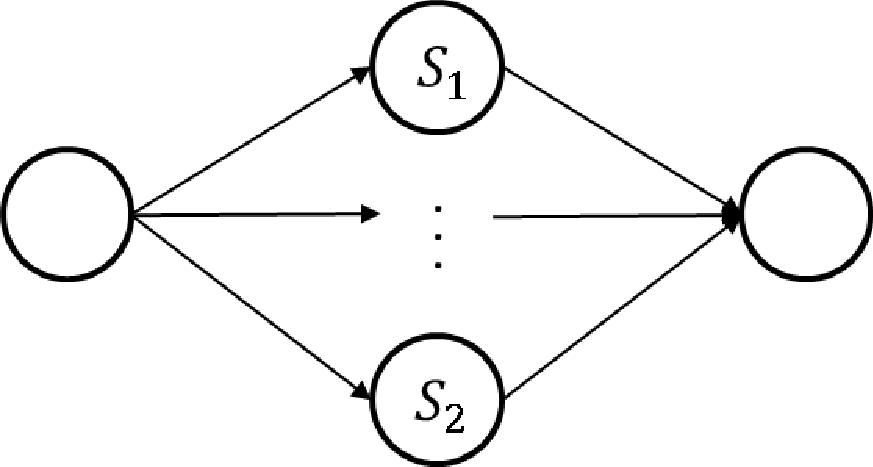
\includegraphics[width=1.4in]{parallel.pdf}\hfill\space\\[0.2cm]
\space\hfill$T=MAX\{t_n|n\in\{1,\ldots,m\}\}$\hfill\space\\[0.2cm]
$C=\sum\limits^m_{n=1}c_n$ \hfill $A=\prod\limits^m_{n=1}a_n$ \hfill
$R=\prod\limits^m_{n=1}r_n$
\end{tabular}}}
\caption{Parallel construct and calculation of its QoS properties
\cite{yu2013adaptive}.}
\label{parallel}
\end{figure}

\subsubsection{Sequence construct}
The composite web service executes each atomic service associated with a sequence construct in a definite sequence order. The aggregation value for total time ($T$) and total cost ($C$) is as the sum of time and cost of web services involved respectively. The overall availability and reliability in a sequence construct are calculated by multiplying their corresponding availability and reliability of each web service in probability theory. This construct is shown in Fig. \ref{sequence}.
\subsubsection{Parallel construct}
Web services in a parallel construct are executed in the meantime. The QoS aggregation value for total cost, availability and reliability are the same as these in sequence construct while the Total time ($T$) is delimited by the maximum time consumed path in the composite flow of the solution. This construct is presented in Fig. \ref{parallel}.

\section{Comprehensive quality-aware Semantic Automated Web Service Composition}\label{qswsc_approach}
\begin{figure}[h]
\centerline{
\fbox{
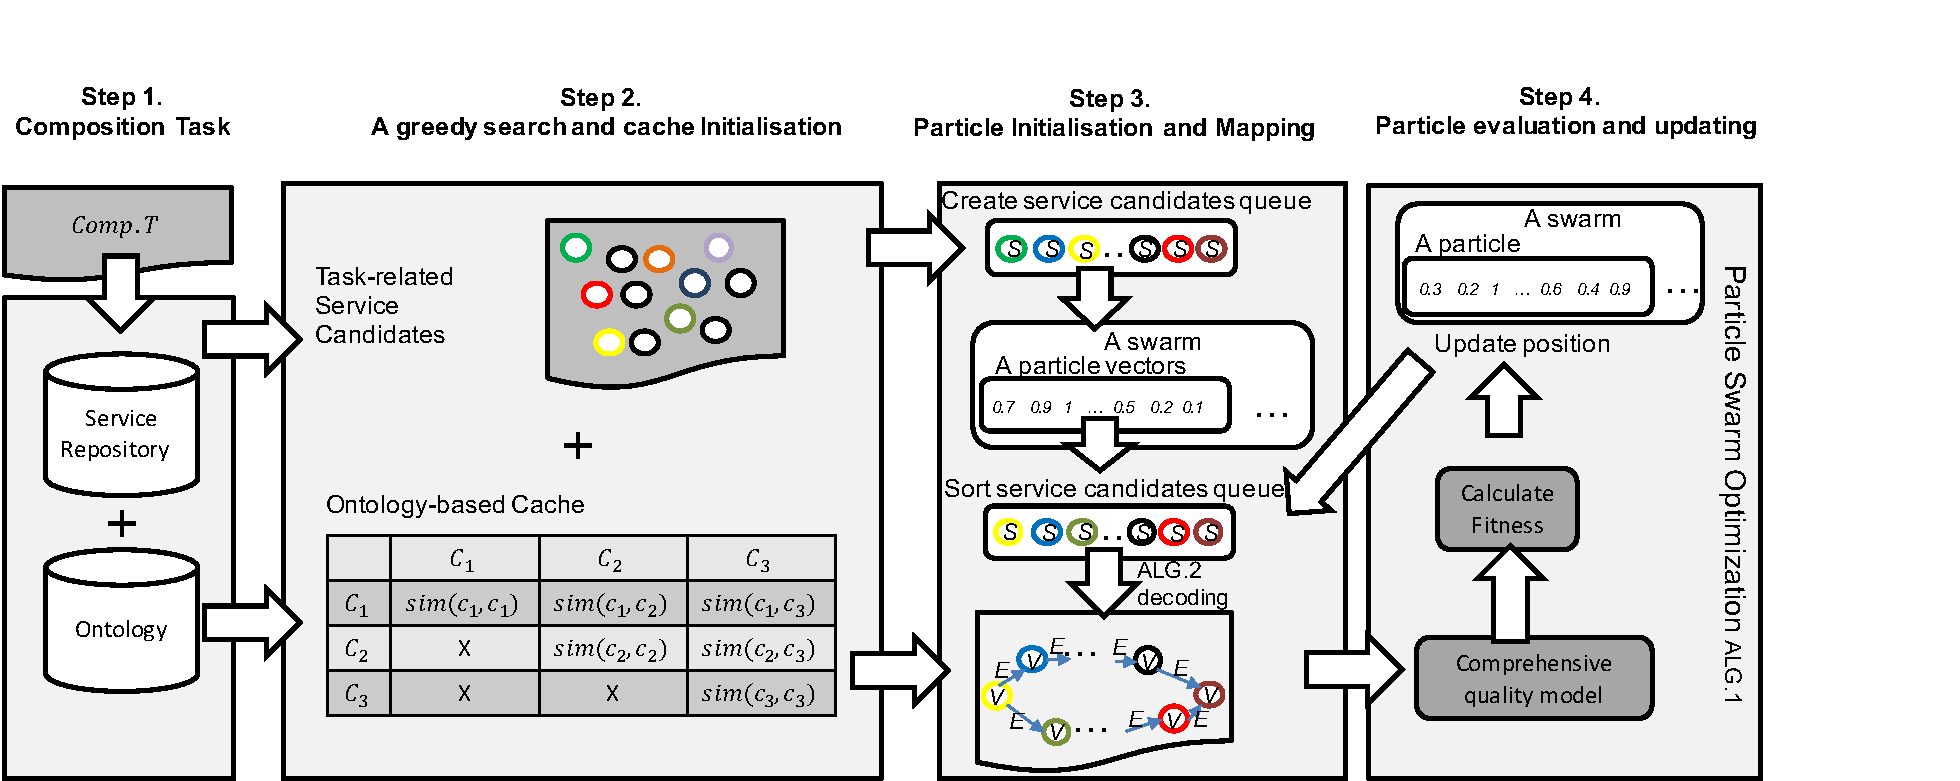
\includegraphics[width=12cm]{overview.pdf}}}
 \caption{Overview of the proposed approach.}
 \label{overview}
\end{figure}
In this paper, we propose a comprehensive quality model for automated semantic service composition, and optimise both the quality of semantic matchmaking and QoS. PSO has shown its efficiency in solving combinatorial optimisation problems. Therefore, we will employ a PSO-based approach, which is considered to be simple and efficient without penalising or repairing comparing to GP \cite{da2014graph}. Fig. \ref{overview} shows the overview of our approach with five steps. Step 1: The composite process is triggered by a composite goal defined in Subsection \ref{problemDes}, which describes customers requirements both functional and non-functional. A functional requirement is defined as $F(T_{Input}, T_{Output})$ , and a nonfunctional one is users' accepted level of QoS. Step 2: Those requirements are used to discover all relevant web services, which leads to a shrunken service repository that further used by PSO as a searching space. Step 3: A weighted graph representation is randomly built up interleaving with semantic matchmaking process, where web services are discovered as graph vertices while edges are assigned with semantic matchmaking quality as weights. Step 4,5: The selection of web services performs PSO algorithm in Sect. \ref{pso_algorithm} to find best particle location. Overall, this approach is different from \cite{da2016particle}, as we use weighted graphs as particle presentation while considering a comprehensive quality.

\subsection{Semantic Matchmaking} \label{semantic_matchmaking}
To perform semantic matchmaking, we transfer a function match between $S_{1}: S_{output} \in C_{1}$ and $S_{2}:S_{output} \in S_{b}$ to a pair of concept match in \ref{semantic Web service Discovery}. The matching process attempts to determine semantic matching between the source concepts of $C_{1}$ and the target concepts of $C_{2}$. Meanwhile, the quality of matched concepts are calculated in the mode model in subSection \ref{qualityModel}. The purpose of semantic matchmaking is to find more component services that could also potentially satisfies the quality of QoS with considering its functional quality.

The semantic matchmaking is achieved by utilising OWL2 and OWL-S or other semantic markup languages for web services. In this paper, we use MECE (Mediation Contract Extension) \cite{bleul2008self} and OWL-DL, MECE is considered to be an alternative semantic annotation for WSDL. MECE defines the service-related inputs and outputs with parameter-related concepts. OWL-DL is a sublanguage of OWL from extension of RDF. which specifies semantic information of concepts involved in MECE. 

\subsection{Comprehensive Quality Model and Aggregation Matrix}\label{qualityModel}
In this paper, we propose a comprehensive quality model to evaluate the overall quality of semantic web service composition. This model overcome the disadvantages of current prevailing QoS-aware optimisation, in which quality of semantic matchmaking are not considered \cite{bansal2016generalized,mier2015integrated,da2016particle,da2015graphevol,yu2013adaptive}.

\textbf{Semantic matchmaking model}. Due to the discretisational characteristics of different match types driven by the cost of  data type integration and manipulation \cite{lecue2009optimizing}, match types are considered to be one factor for the semantic matchmaking quality. Another factor in our proposed model is concept similarity, which could be evaluate based on edge counting method defined by \cite{shet2012new}, which is a taxonomy-based measurement for ontology matching. This formula \ref{equation1} is used to estimate the similarity between parameter-related output concept and parameter-related input concept for selecting web services. Therefore, given the quality match type and the similarity of two parameters-related concepts, the semantic matchmaking quality of matched parameters is defined by Formula \ref{equation2}, where the value of $q(p_ {matchType})$ is set up as the same as the quality of the semantic link in \cite{lecue2009optimizing} as 1 (Exact), 0.75 (Plugin), 0.5 (Subsume) or 0.25 (Intersection). 

\begin{equation}
q(p_ {s}){=} \frac{2N \cdot e^{-\lambda L/D} }{N_{1}+N_{2}}
\label{equation1}
\end{equation}

\begin{equation}
\label{equation2}
q(p_{sm}) \stackrel{.}{=} (q(p_ {mt}), \  q(p_ {s}))
\end{equation}

Further more, edges represent services connections in our weighted graph presentations, where assigned weight value $q(e_{sm})$ is considered to be semantic matching quality on edge level according to parameter aggregations. The weight value $q(e_{sm})$ is defined in \ref{equation3}, where $q(e_ {matchType})$ and $q(e_ {similarity})$ are the mean value of concept-related parameters quality in $q(p_{mt})$ and $q(p_{s})$ respectively. 

\begin{equation}
\label{equation3}
q(e_{sm}) \stackrel{.}{=} (q(e_ {mt}), \  q(e_ {s}))
\end{equation}

\textbf{Comprehensive quality model}. Compared to QoS evaluation model, the comprehensive quality model is established to investigate both functional and non-functional requirements of a goal. The comprehensive quality of our service composition representation refers to QoS of service vertices and Semantic matching quality of Edges in weighted graphs. Consequently, the comprehensive quality model is defined in Formula \ref{equation4}, which could be further broken down into Formula \ref{equation5}. 
\begin{equation}
\label{equation4}
q_{cq} \stackrel{.}{=} (q(e_ {sm}), \  q(v_ {QoS}))
\end{equation}
\begin{equation}
\label{equation5}
q_{cq} \stackrel{.}{=} (q(e_ {mt}), \  q(e_ {s}), \  q(v_{a}),\  q(v_{r}),\  q(v_{c}),\  q(v_{t}))
\end{equation}

\textbf{Quality aggregate matrix}. The quality aggregation is defined based on the constructs of composite web services on the criteria of functional and non-functional properties. The quality on construct level is further calculated and by following the rules summarised in Table \ref{table1}. 

% Please add the following required packages to your document preamble:
% \usepackage{multirow}
\begin{table}[]
\centering
\caption{Quality aggregate matrix for semantic web service composition}
\label{table1}
\begin{tabular}{|c|c|c|c|l|}
\hline
\multicolumn{3}{|c|}{Composition Construct}                                      & Sequence                             & Parallel \\ \hline
\multirow{5}{*}{QualityFactors} & \multirow{2}{*}{Functional}    & $Q(e_ {mt})$  &$\prod_{n=1}^{m} q(e_ {mt})$          &  $\prod_{n=1}^{m} q(e_ {mt})$ \\ \cline{3-5}
                                &                                & $Q(e_ {s})$  & $(\sum_{n=1}^m q(e_ {s}))/m$        &  $(\sum_{n=1}^m q(e_ {s}))/m$  \\ \cline{2-5}   
                                & \multirow{4}{*}{NonFunctional} & $Q(v_{a})$    & $\prod_{n=1}^{m} q(v_a)$             &  $\prod_{n=1}^{m} q(v_a)$ \\ \cline{3-5} 
                                &                                & $Q(v_{r})$    & $\prod_{n=1}^{m} q(v_r)$             &  $\prod_{n=1}^{m} q(v_r)$ \\ \cline{3-5} 
                                &                                & $Q(v_{c})$    & $\sum_{n=1}^m q(v_ {c})$             &  $\sum_{n=1}^m q(v_ {c})$ \\ \cline{3-5} 
                                &                                & $Q(v_{t})$    & $\sum_{n=1}^m q(v_ {t})$             &  $max(q(v_ {t}))$ \\ \hline
\end{tabular}
\end{table}



\subsection{Composition Weighted Graph}
We defined our semantic web service composition solution as $WG = (V, E)Graph$, where $V$ is a set of services as vertex: $V=[S1, S2...Sn]$ and $E$ is a set of edges $E = {e_{1}, e_{2},... e_{n}}$. Each $e$ is associated with $q(e_{sm})$ as weight value that mapped to a pair of quality values $q(e_{mt})$ and $q(e_{s})$ on the edge level. where $e_{m}$ is expressed as $(S_{a},S_{b})={q_{mt}, q_{s}}$. Here we provide an example of the web service composition, which can be described in the Fig. \ref{wscs}. The data of composite web service flows from the start to the end, where five web services involved and linked with each other using edge connections. Besides that, $q(s_{mt})$ and $q(s_{s})$ are calculated for all edges ${e_{1}, e_{2},... e_{n}}$, and further aggregated in $Q_{mt}$ and $Q_{s}$ respectively on the construct level. In addition, $Q_{QoS}$ is calculated by all the non-functional attributes of $V$ using aggregation rules defined previously.

\begin{figure}[h]
\centerline{
\fbox{
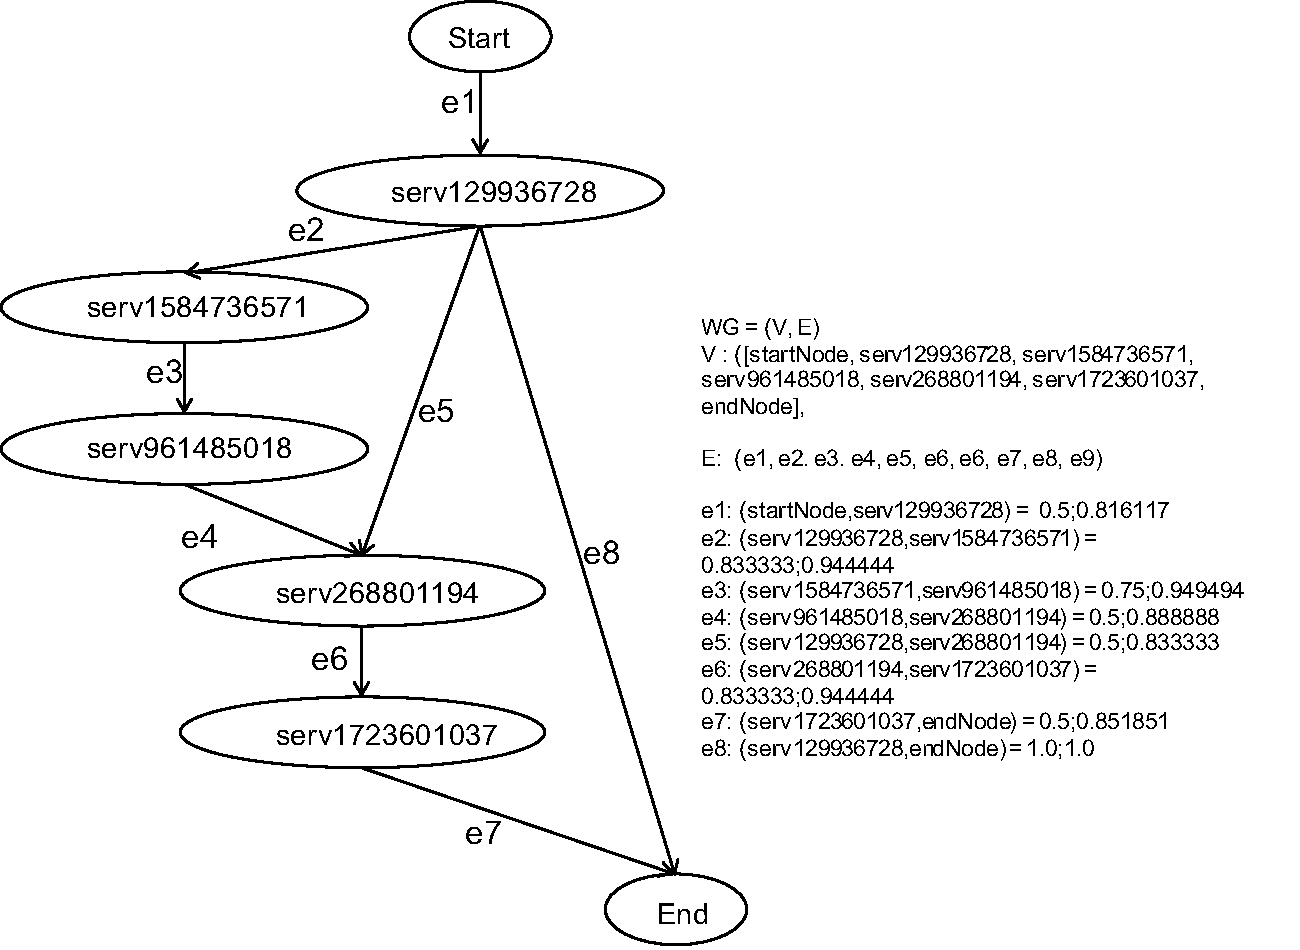
\includegraphics[width=8cm]{weigtedGraphExample.pdf}}}
 \caption{Composition weighted graph solution}
 \label{wscs}
\end{figure}

\subsection{Fitness Calculation}
The fitness value of a service composition solution is a weighted sum of all the quality components discussed previously shown in Formula \ref{equation6}, in which fitness value of 1 means the best comprehensive quality and 0 means the worst. As the sum of all the components' weights ($w_1$ to $w_6$) equals to 1, $MT$, $S$, $A$, $R$, $T$, and $C$ must be normalised so that the fitness value falls within the range from 0 to 1. Also, the lowest T and C value represent the best component quality so that the objective function can be offset using $(1 - T)$ and $(1 - C)$ using normalisation formula \ref{equation8}, and normalisation formula \ref{equation7} is for the rest components. Therefore, the whole problem is treated as a maximisation problem.

\begin{equation}
\label{equation6}
Fitness = w_1MT + w_2S + w_3A + w_4R + w_5(1 - T) + w_6(1 - C)
\end{equation}
\noindent where $\sum_{i=1}^{6} w_i = 1$
\\\\
\begin{equation}
\label{equation7}
normalise(value) = 
\begin{cases}
	\frac{value - min}{max - min} & \text{ if }max - min \neq 0.\\
	1 & \mathrm{ otherwise}.
\end{cases}
\end{equation}
\begin{equation}
\label{equation8}
normalise(value) = 
\begin{cases}
	\frac{max - value}{max - min} & \text{ if }max - min \neq 0.\\
	1 & \mathrm{ otherwise}.
\end{cases}
\end{equation}


\subsection{QoS-aware Semantic Web Service Composition Algorithm} \label{pso_algorithm}

\begin{algorithm}[!htb]
 \setlength\hsize{0.9\linewidth}
 \SetKwInOut{Input}{Input}\SetKwInOut{Output}{Output}
 \let\oldnl\nl% Store \nl in \oldnl
\newcommand{\nonl}{\renewcommand{\nl}{\let\nl\oldnl}}
 \LinesNumbered
 	\textbf{1.} Map each relevant service to an index in the particle's position vector.\\
	\textbf{2.} Randomly initialise each particle in the swarm.\\
	\nonl \While {max. iterations not met}{
		\ForAll{particles in the swarm}{
		    \textbf{3.} Create queue of services using the particle's position vector.\\
			\textcolor{blue}{\textbf{4.} Build a weighted graph using the queue.}\\
			\textcolor{blue}{\textbf{5.} Calculate the fitness of the weighted graph.}\\
			\eIf{fitness value better than pBest}{
				\textbf{6a.} Assign current fitness as new pBest.\\
			}{
				\textbf{6b.} Keep previous pBest.\\
			}		
		}
		\textbf{7.} Assign best particle's pBest value to gBest, if better than gBest.\\
		\textbf{8.} Calculate the velocity of each particle according to the equation:\\
		\Indp $v_{id} = v_{id} + c_1 * rand() * (p_{id} - x_{id}) + c_2 * rand() * (p_{gd} - x_{id})$\\
		\Indm \textbf{9.} Update the position of each particle according to the equation:\\
		\Indp $x_{id} = x_{id} + v_{id}$\\
	}
	
 \caption{Steps of the PSO-based Web service composition technique.}
\label{novelSteps}
\end{algorithm}

\begin{algorithm}[!htb]
 \setlength\hsize{0.9\linewidth}
 \SetKwInOut{Input}{Input}\SetKwInOut{Output}{Output}
 \let\oldnl\nl% Store \nl in \oldnl
\newcommand{\nonl}{\renewcommand{\nl}{\let\nl\oldnl}}
 \Input{$I$, $O$, $queue$}
 \Output{composition weighted graph $WG$}
 \textbf{1.} Create $start$ vertex with outputs $O$ and $end$ vertex with inputs $I$.\\
 \textbf{2.} Create graph $WG$ containing the $start$ vertex.\\
 \textbf{3.} Create available outputs set containing $start$ outputs.\\
 \While{available outputs do not satisfy $end$ inputs}{
 \textbf{4.} Get next candidate from queue.\\
 \If{candidate inputs are satisfied by available outputs}{
 \textcolor{blue}{\textbf{5.} Create edge assigned with weight.\\}
 \textcolor{blue}{\textbf{6.} Connect vertex to graph with the edge.\\}
 \textbf{7.} Remove it from queue and go back to the queue's beginning.\\
 }}
 \textbf{8.} Connect end vertex.\\
 \textbf{9.} Remove dangling vertices from graph $WG$.\\
 \textcolor{blue}{\textbf{10.} Remove dangling edges from graph $WG$.\\}
 \KwRet $WG$.\\
 \caption{Create a composition weighted graph from a queue}	
\label{graph_building}
\end{algorithm}

The overall algorithm investigated here is a PSO-based web service composition algorithm \ref{novelSteps} from   \cite{da2016particle} with a different decoded algorithm \ref{graph_building} to generate a composition weighted graph from a queue. In the first algorithm, the idea is to translate the particle location into a service queue as an indirect representation of composition weighted graph, so finding the best fitness of the composite weighted graph is to discover the optimised location of the particle in the search space. In PSO, the dimension of the particle is set up as the same number as relevant web services, and the index of services is mapped to the location vectors in a particle, and we put services in a queue in ascending order, from which we decode a weighted graph using Algorithm \ref{graph_building}. We select and connect  service vertex to the start vertex from the service queue if the web service can satisfy the output of start vertex. Meanwhile, an Output Set is initialised and kept being updated using outputs from the new-added service vertex in the weighted graph, later on, more services vertex are connected with edges if services' inputs could be satisfied by any output in the Output Set. At last, The end vertex is connected if the updated Output Set contains all end inputs. In addition, dangling service vertex and edges should be removed. 

\section{Experiment Design}\label{experiment_design}
In this section, a quantitative evaluation approach is adopted in our experiment design. The objectives of the evaluation are $(1)$ to measure the effectiveness of the comprehensive quality model in automated semantic web service composition approach, $(2)$ to explore the impacts of the semantic matchmaking that contributes to overall composition quality, and $(3)$ to compare solutions generated by QoS-ware approach with our method.

We utilise benchmark dataset web service challenge 2009 (WSC09) \cite{kona2009wsc} to perform a evaluation. WSC09 provides problems where five tasks consisted in with variable size in both services, and ontologies. Therefore, it is a proper dataset for the scalability measures in our defined quality evaluation model. Table \ref{wsc09datasetTable} presents the features of the WSC’09 dataset. The number of concepts, individuals in the ontology and services in each data set is shown in the second, third, fourth column respectively. Also, we extend all the datasets with QoS attributes from service providers to enable our evaluation. 
\begin{table}[]
\centering
\caption{Features of the WSC09 datasets}
\label{wsc09datasetTable}
\begin{tabular}{|l|l|l|l|}
\hline
\multicolumn{1}{|c|}{Dataset} & No.Concept & No.Individual & No.Service \\ \hline
WSC09 01                     & 1578       &3102           &572      \\ \hline
WSC09 02                     & 12388      &24815          &4129      \\ \hline
WSC09 03                     & 18573      &37316          &8138      \\ \hline
WSC09 04                     & 18673      &37324          &8301      \\ \hline
WSC09 05                     & 31044      &62132          &15211    \\ \hline
\end{tabular}
\end{table}


We run the experiment under computing grid comprising of almost 170 NetBSD (Unix operating system) workstations operated by the Sun Grid Engine. Experimentation is done using the approach explained in Section \ref{qswsc_approach}, and evaluated in the comprehensive quality model introduced in Subsection \ref{qualityModel}. The parameters were chosen based on general settings from \cite{shi2001particle} for our PSO-based approach, 30 particles evolved in 100 generations in the searching space, in which problem dimension's size equals to the number of relevant services in service repository. We run 30 times independently for each dataset. In addition, weight settings are flexibly defined by users' preferences. As part of their requirement, we configure weight of fitness function to properly balance functional side and nonfunctional side. Therefore, $w_{1}$ and $w_{2}$ are equals to 0.1 and 0.4,  and $w_{3}$, $w_{4}$, $w_{5}$, $w_{6}$ are all set to 0.125 accordingly.

\section{Results and Analysis}\label{results_analysis}
\subsection{Comparison Test}\label{comparisonTest}

In this section, we analyse the composition solution generated by using our approach comparing with QoS-aware approach. In particularly, we show that our proposed approach can produce solutions that results better matchmaking , which meets user's goal better. In particularly, we look at mean value of $Q_{mt}$, $Q_{s}$ and $Q_{QoS}$ in the comprehensive quality awareness approach and QoS awareness approach are compared to reveal how good our evaluation mode in Table \ref{decisionTable}. In each task, we compare $Q_{mt}$, $Q_{s}$ and $Q_{QoS}$, and $Q_{QoS}$ is normalised to make it comparable to another method in our comprehensive awareness approach 

% Please add the following required packages to your document preamble:
% \usepackage{multirow}
\begin{table}[]
\footnotesize
\centering
\caption{Mean Quality for comprehensive quality-aware methods and QoS-aware appraoch}
\label{decisionTable}
\begin{tabular}{|c|c|c|c|}
\hline
\multicolumn{2}{|c|}{}                                               & \shortstack{QoS-aware \\ Evaluation} & \shortstack{Comprehensive \\ Quality Evaluation} \\ \hline
\multirow{3}{*}{Task1}  &$Q_{mt}$   & .232635              & .232635                          \\ \cline{2-4} 
                                      &$Q_{s}$                       & .903572              & .903572                          \\ \cline{2-4}
                                      &$Q_{QoS}$                     & .578577              & .578577                          \\ \hline
\multirow{3}{*}{Task2}  &$Q_{mt}$   & .001828              & .000851$\downarrow$               \\ \cline{2-4} 
                                      &$Q_{s}$                       & .917172              & .938840$\uparrow$                 \\ \cline{2-4}
                                      &$Q_{QoS}$                     & .480251              & .473002$\downarrow$               \\ \hline
\multirow{3}{*}{Task3}  &$Q_{mt}$   & .191188              & .247836$\uparrow$                  \\ \cline{2-4} 
                                      &$Q_{s}$                       & .951509              & .973723$\uparrow$                  \\ \cline{2-4}
                                      &$Q_{QoS}$                     & .493927              & .491538$\downarrow$                 \\ \hline
\multirow{3}{*}{Task4}  &$Q_{mt}$   & .919678              & .943406$\uparrow$                  \\ \cline{2-4} 
                                      &$Q_{s}$                       & .000000              & .000009$\uparrow$                  \\ \cline{2-4}
                                      &$Q_{QoS}$                     & .480818              & .472485$\downarrow$                 \\ \hline
\multirow{3}{*}{Task5}  &$Q_{mt}$   & .000094              & .000109$\uparrow$                  \\ \cline{2-4} 
                                      &$Q_{s}$                       & .927476              & .930975$\uparrow$                  \\ \cline{2-4}
                                      &$Q_{QoS}$                     & .476236              & .475128$\downarrow$                 \\ \hline                                                   
\end{tabular}
\end{table}
In Table \ref{decisionTable}, Task 1 represents the same solution using different methods where the values of $Q_{mt}$,$Q_{s}$ and $Q_{QoS}$ are all the same. It is due to the size of dataset 01 is very small in both available services and ontologies. However, As the size of dataset increase, we can recognise a trade-offs in task 2 using our evaluation approach, where a 0.021668 increase in similarity quality and a 0.00098 decrease in matchType quality with weights 0.4 and 0.1 respectively so that solution to task 2 is still considered to be an improvement in the functional quality part while a decrease value of 0.007249 in QoS. In task 3, the benefit of functional part quality is clearer with an increase value of 0.056648 and 0.078862 in  similarity quality and matchType quality respectively while a slight decrease in QoS. later on, the rest tasks perform the same behaviour in $Q_{mt}$,$Q_{s}$ and $Q_{QoS}$ as task 3. In conclusion, we can perceive that our evaluation could find out better functional quality with a reasonable trade off in QoS.

To visually compare the results generated from two evaluation approaches, we demonstrate the differences in the solutions of two composition weighted graphs under two different methods. The Fig. \ref{comparison} shows two composition weighted graphs, which are the solutions to Task 3 for(1) QoS-aware approach and $(2)$ Comprehensive quality-aware method and respectively. It can be observed that two composition weighted graphs have exactly the same workflow structure, in which the same service vertex and edges are different denoted in red. Meanwhile, we make a comparison of those different edges weights representing the quality of semantic matchmaking in Table \ref{comparisontable},as well as QoS. We can see edges obtain better semantic matchmaking quality with a reasonable trade-off in QoS



\begin{figure}[h]
\centerline{
\fbox{
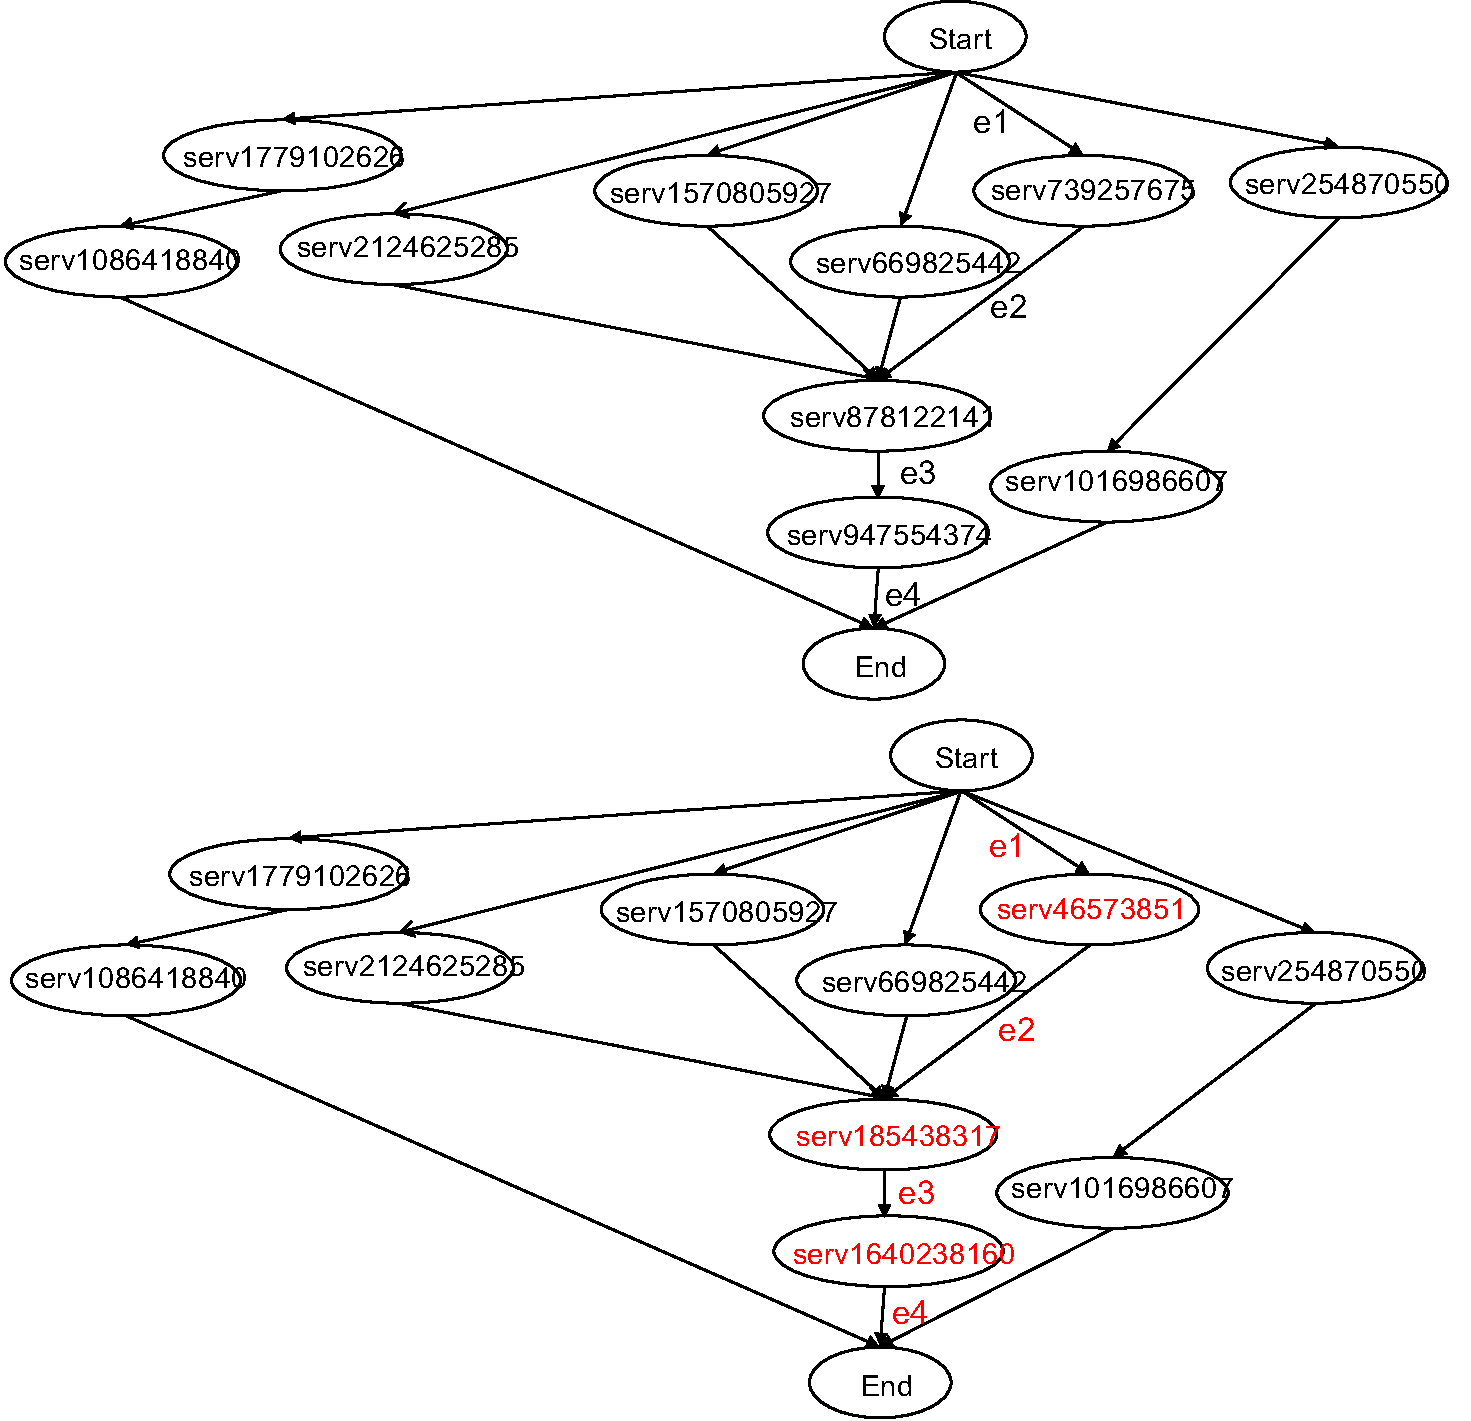
\includegraphics[width=8cm]{comparision.pdf}}}
 \caption{Example Comparison of solutions to Task 3 under different approaches.}
 \label{comparison}
\end{figure}

% Please add the following required packages to your document preamble:
% \usepackage{multirow}
\begin{table}[]
\centering
\caption{Comparison of Composition Weighted Graphs}
\label{comparisontable}
\begin{tabular}{|l|l|l|l|l|}
\hline
\multicolumn{2}{|l|}{Quality criteria} & Weighted Graph $(1)$ & Weighted Graph $(2)$ &  $\Delta Q$\\ \hline
\multirow{2}{*}{e1} &$q(e_{mt})$   &1        &1                       &0     \\ \cline{2-5} 
                    & $q(e_{s})$   &1        &1                       &0\\ \hline
\multirow{2}{*}{e2} & $q(e_{mt})$  &0.75     &0.9167                  &+0.1667 \\ \cline{2-5} 
                    & $q(e_{s})$   &0.9232   &0.9630                &+0.0398\\ \hline
\multirow{2}{*}{e3} &  $q(e_{mt})$ &0.75     &0.8333                 &+0.08333\\ \cline{2-5} 
                    &   $q(e_{s})$ &0.8230   &0.9608                 &+0.1378\\ \hline
\multirow{2}{*}{e4} & $q(e_{mt})$  &0.75     &0.875                  &+0.125\\ \cline{2-5} 
                    &  $q(e_{s})$  &0.9090   &0.9167                 &+0.0077\\ \hline
\multicolumn{2}{|l|}{QoS} &0.4949            &0.4915                 &-0.0034  \\ \hline
\end{tabular}
\end{table}

\subsection{Convergence Test}\label{convergenceTest}

\begin{figure}[h]
\centerline{
\fbox{
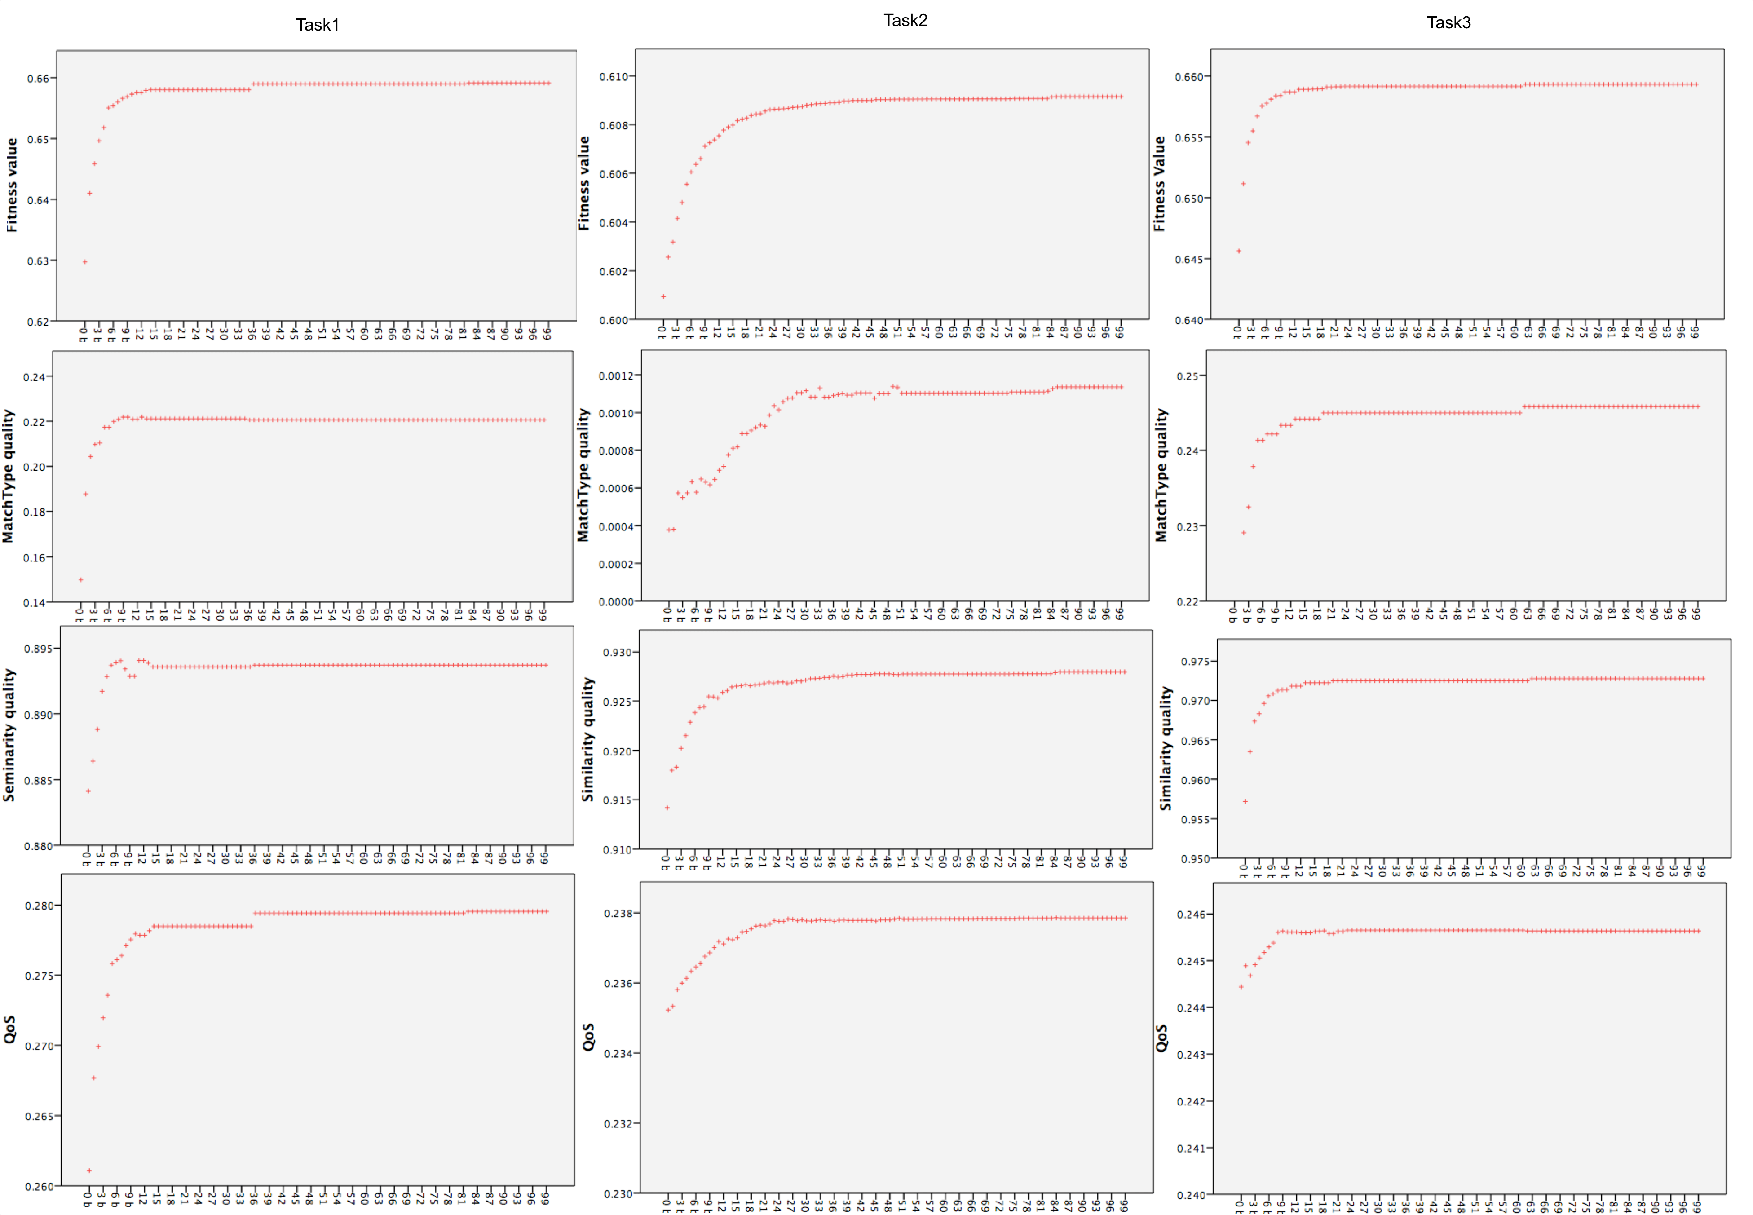
\includegraphics[width=12cm]{convergency.pdf}}}
 \caption{Average Fitness, Average MatchType Quality, Average Similarity quality and Average QoS per generation with comprehensive quality optimum}
 \label{exp_fitnessvalue}
\end{figure}

To analyse the effectiveness of our approach, we will study the convergence rate of the proposed method in this section to understand the convergence rate of five tasks in WSC09. To further study the overall effectiveness of evaluation model and explore impacts of all involved components in the fitness function. We analysis all the performances of these components in the whole evolutionary process in Fig. \ref{exp_fitnessvalue}, in which the five tasks' experiment results are arranged in four groups consisting of average fitness, average matchType quality, average similarity quality and average QoS for generation 0-99 with optimum.

Firstly, the average fitness value with optimum is calculated by the average value of best fitness found in each generation over 30 independent runs. The value plotted in the first column group ranges from 0 to 1 in Fig. \ref{exp_fitnessvalue}, and it is considered to be more optimised if its value is closer to value 1. We can see that there is a significant increase in the fitness values with optimum between generation 0 and generation 15-25, the remaining generation continues to produce a steady but moderate improvement in the fitness value and eventually reach a plateau with no further changes. The same behaviour is observed over the rest tasks. We also witnessed a fast convergence rate of the fitness value.

We also investigate the variation of quality of semantic matchmaking where average matchType quality with optimum and average similarity quality with optimum are studied from generation 0 to 99 in second and third column groups of Fig. \ref{exp_fitnessvalue}. In these groups,  both the average matchType quality with optimum and average similarity quality with optimum are the mean value corresponding to the best fitness value found in each generation over 30 independent runs. The dominant tendency of the marked value representing a similar characteristic compared to the average fitness value group trend in five tasks. However, there are some slight fluctuations over the generations.

Lastly, it is interesting to look at the average QoS per generation for the 30 independent runs when the functional quality heads up. Here average QoS with optimum is also the value corresponding to the fitness value with optimum in each generation, and we display the results in the fourth column group in Fig. \ref{exp_fitnessvalue}. It is obvious that the overall trend of QoS moves upward to a high constant level in five independent tasks. Additionally, we don't see too much trade-off from the QoS.


\section{Conclusion}\label{conclusion}
This work introduced a evaluation model for QoS-aware automated semantic automated web service composition that is based on a semantic matchmaking quality extends existing QoS. The results shows that our comprehensive quality model is proved to obtain better functional quality with a reasonable trade-off in QoS. Future works in this area could explore the comprehensive quality with multi-objectives to maximising quality of matchmaking and to optimise QoS, and improve efficiency in calculating semantic quality.
\bibliographystyle{splncs03}
\bibliography{bibliography}

\end{document}